\documentclass[conference]{IEEEtran}
\IEEEoverridecommandlockouts
% The preceding line is only needed to identify funding in the first footnote. If that is unneeded, please comment it out.
\usepackage{cite}
\usepackage{amsmath,amssymb,amsfonts}
\usepackage{algorithmic}
\usepackage{graphicx}
\usepackage{listings}
\lstset{breaklines=true}
\usepackage{url}
\graphicspath{ {images/} }
\usepackage{textcomp}
\usepackage{xcolor}
\def\BibTeX{{\rm B\kern-.05em{\sc i\kern-.025em b}\kern-.08em
    T\kern-.1667em\lower.7ex\hbox{E}\kern-.125emX}}


\begin{document}

\title{Smart City: Networked traffic controller for autonomous vehicle\\
{\footnotesize }
}

\author{\IEEEauthorblockN{1\textsuperscript{st} Sheikh Muhammad Adib \\Bin Sh Abu Bakar}
\IEEEauthorblockA{\textit{Fachhochschule Dortmund} \\
\textit{ME. Embedded Systems Engineering}\\
sheikh.binshabubakar001@stud.fh-dortmund.de}

\and
\IEEEauthorblockN{2\textsuperscript{nd} Mohammed Rizwan }
\IEEEauthorblockA{\textit{Fachhochschule Dortmund} \\
\textit{ME. Embedded Systems Engineering}\\
mohammed.mohammedrizwan009@stud.fh-dortmund.de}

\and
\IEEEauthorblockN{3\textsuperscript{rd} Aditya Kumar}
\IEEEauthorblockA{\textit{Fachhochschule Dortmund} \\
\textit{ME. Embedded Systems Engineering}\\
aditya.kumar001@stud.fh.dortmund.de}

\and
\IEEEauthorblockN{4\textsuperscript{th} Farhaad Sheikh Mohammed}
\IEEEauthorblockA{\textit{Fachhochschule Dortmund} \\
\textit{ME. Embedded Systems Engineering}\\
farhaad.sheikhmohammed002\\@stud.fh-dortmund.de}
\and

\IEEEauthorblockN{5\textsuperscript{th} Mykyta Konakh}
\IEEEauthorblockA{\textit{Fachhochschule Dortmund} \\
\textit{ME. Embedded Systems Engineering}\\
mykyta.konakh001@stud.fh-dortmund.de}
}

\maketitle



\begin{abstract}
This paper presents the design, implementation, and validation of a networked traffic control system for autonomous vehicles for traffic management in smart cities, outlining requirements, architecture, processes, hazards, and solutions.
\end{abstract}

\begin{IEEEkeywords}
Smart city, Traffic controller, Autonomous vehicle
\end{IEEEkeywords}

\section{Introduction}
\label{sec:intoduction}

A smart city is an urban area where technology and data collection improve the quality of life, sustainability, and efficiency of city operations \cite{b1}. Smart city technologies include information and communication technologies (ICT) and the Internet of Things (IoT). These technologies increasingly play a crucial role in areas such as transportation, energy, and infrastructure \cite{b2}. Smart city technologies, such as smart transportation systems, can optimize traffic flow, reduce congestion, and improve the quality of life for city residents and commuters using real-time data. Although implementing such a system, especially with the rise of autonomous vehicles, can be challenging, A networked traffic control system is needed to integrate these vehicles into urban infrastructure. 
This paper explores the design, implementation, and validation of a networked traffic control system for autonomous vehicles in smart cities. It identifies key requirements, use cases, system contexts, and constraints and outlines the architecture, roles, and processes of TCUs (Traffic Controller Units) and RSUs (Road Side Units). The system's performance is evaluated through test cases, and potential risks are identified, including communication failures, software and hardware malfunctions, and power fluctuations. Solutions are proposed to enhance system resilience and safety.

\begin{figure}[ht]
    \centering
    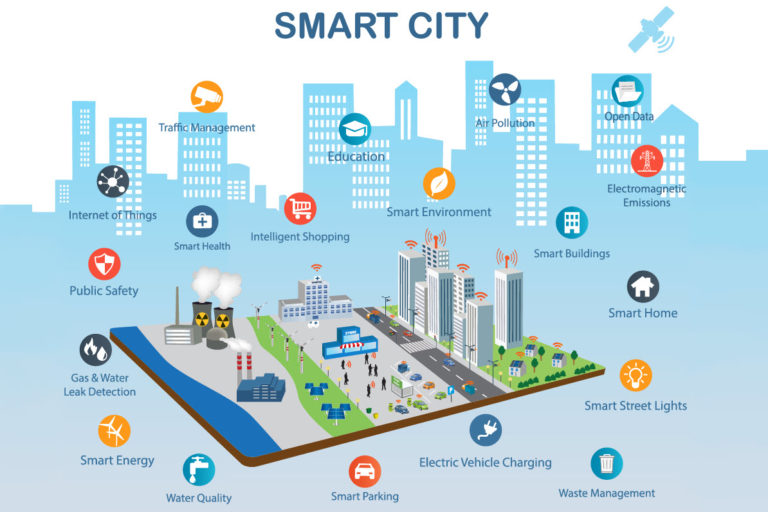
\includegraphics[width=0.5\textwidth]{images/smart-cities-infrastructure-iot-wide-768x512.jpg}
    \caption{Smart City Technologies \cite{b3}}
    \label{img:main_use_case}
\end{figure}

\input{section/03Analysis:use_case}
\input{section/04Analysis:requirements}
\input{section/05Analysis:constraint}
\input{section/06DesignAndImplementation:system_architecture}
\input{section/07DesignAndImplementation:RSUandTCUposition}
\input{section/07DesignAndImplementation:V2I Communication}
\input{section/08DesignAndImplementation:process_1}
\input{section/09DesignAndImplementation:process_2}
\input{section/10DesignAndImplementation:process_3}
\input{section/11DesignAndImplementation:scheduling}
\input{section/12V&V:test_case}
\section{Hazard}
\label{sec:hazard} 

\begin{figure}[ht]
    \centering
    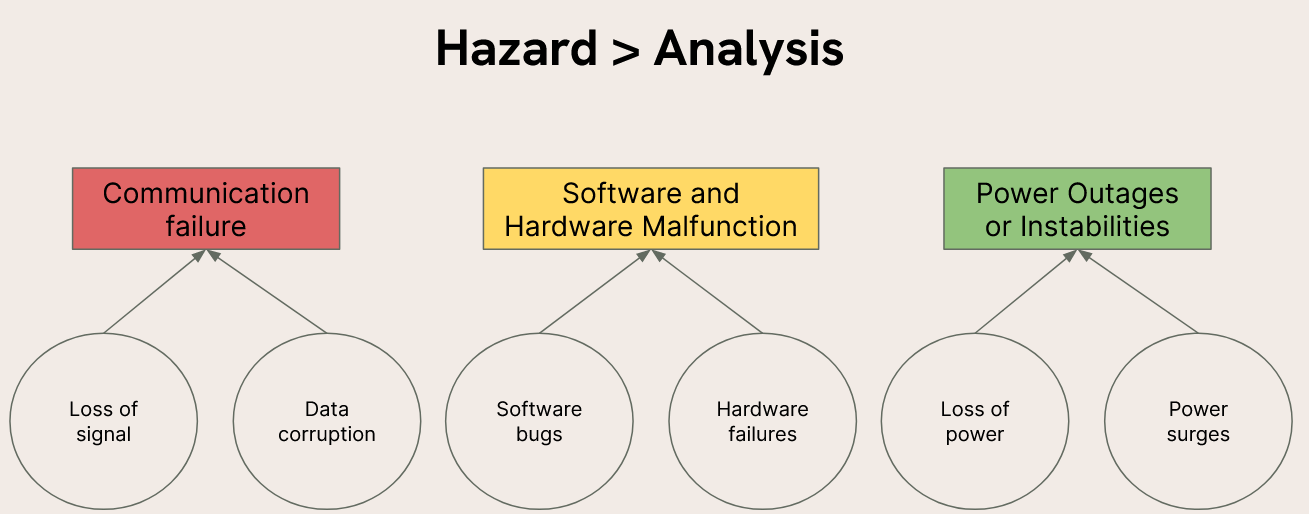
\includegraphics[width=0.5\textwidth]{images/hazard_analysis.png}
    \caption{Diagram outlining the main categories of hazards.}
    \label{fig:hazard_categories}
\end{figure}

The diagram is organized into three main categories of hazards. An overview of the hazards illustrated in Figure \ref{fig:hazard_categories}

\begin{enumerate}
    \item Communication Failure: This category identifies the risks associated with the failure of communication systems. Subcategories include:
    \begin{enumerate}
        \item Loss of Signal: This can mean interruption of communication lines or signals, which can lead to a lack of coordination or response in a critical situation.
        \item Data Corruption: This hazard involves the alteration of data during transmission, which may result in incorrect information and action.
    \end{enumerate}

    \item Software and Hardware Malfunction: This category refers to potential problems with software and hardware components of the system. Subcategories include:
    \begin{enumerate}
        \item Software Bugs: Flaws or errors in software code that can cause unexpected behavior or system failures.
        \item Hardware Failures: Physical malfunctions or breakdowns of hardware components that can cause system malfunctions or improper operations.
    \end{enumerate}

    \item Power Failures or Fluctuations: This category focuses on the power supply and the risks associated with its failures or fluctuations. Subcategories include:
    \begin{enumerate}
        \item Power Loss: Complete power failures that can shut down an entire system or individual critical components.
        \item Power Surges: Power surges that can damage equipment, corrupt data, or cause erratic system behavior.
    \end{enumerate}
\end{enumerate}

\begin{figure}[ht]
    \centering
    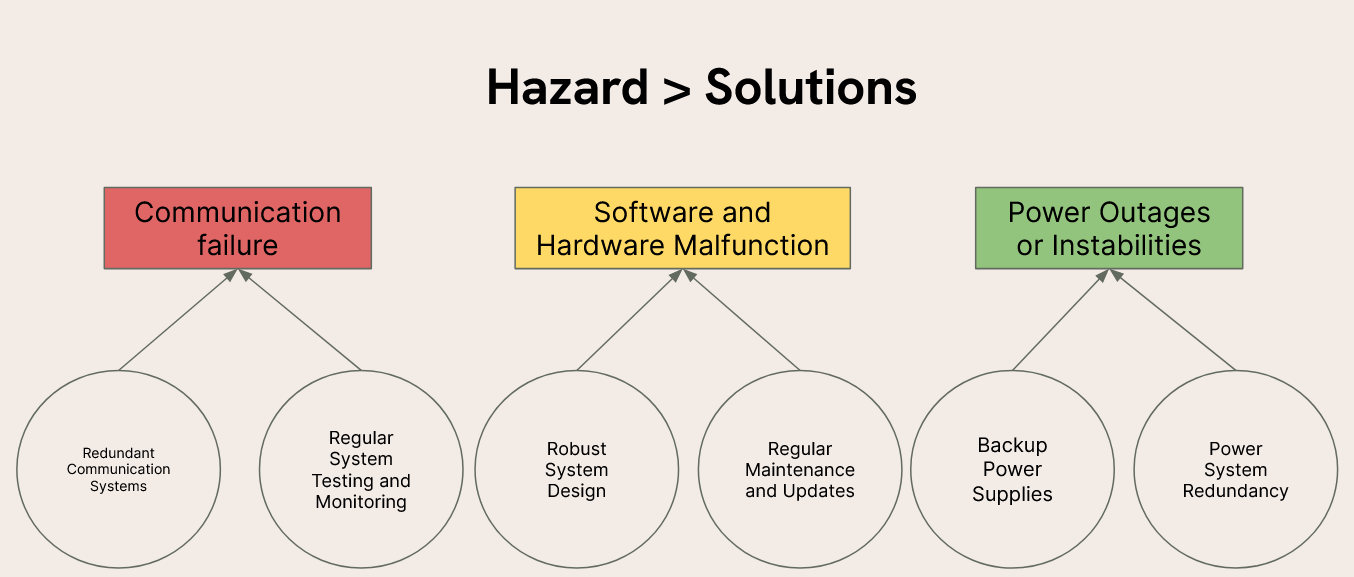
\includegraphics[width=0.5\textwidth]{images/hazard_solutions.png}
    \caption{Solutions to address the identified hazards.}
    \label{fig:hazard_solutions}
\end{figure}

Solutions illustrated in Figure \ref{fig:hazard_solutions}.Solutions to address these hazards include:

\begin{enumerate}
    \item Solutions to Address Communication Failures:
    \begin{enumerate}
        \item Redundant Communication Systems: Implementing redundant systems ensures continuous and reliable communication by having backup channels or methods that can take over in case the primary communication path fails.
        \item Regular System Testing and Monitoring: Regular testing and monitoring of communication systems help detect and correct faults before they lead to failure, thus preventing signal loss or data corruption.
    \end{enumerate}

    \item Solutions for Software and Hardware Faults:
    \begin{enumerate}
        \item Robust System Design: A robust system design includes using high-quality components, developing fault tolerance, and implementing error-handling procedures to prevent complete system failure if a component fails.
        \item Regular Maintenance and Updates: Regular maintenance and software updates can address hardware problems and software bugs, preventing them from leading to failures.
    \end{enumerate}

    \item Solutions for Power Outages or Instabilities:
    \begin{enumerate}
        \item Backup Power Supplies: Backup power solutions, like Uninterruptible Power Supplies or generators, provide immediate power to ensure that critical components remain operational during outages.
        \item Power System Redundancy: Power system redundancy, involving alternative power sources or redundant power delivery paths, ensures the availability of power to critical system components at all times.
    \end{enumerate}
\end{enumerate}

\section{Summary and Outlook}
\label{sec:summary_and_outlook} 

In this paper we have discussed how we develop out system prototype from refining our system use case and  designing the system to the simulation of the system behaviour partially for verification and validation. We also consider the Hazards to improve system safety. Since there are many domains that need to be explored where it is beyond our ability, the system we designed has many flaws such as not considering communication failure. However, we focus on our approach to building a system. In the future, many stake holder shall involve in this project to improve the system requirement,thus improve the system design to make it more dependable.
\begin{thebibliography}{00}
\bibitem{b1}Team, L. (2023, March 10). How IoT is enhancing the development of smart cities. Lvivity. https://lvivity.com/iot-and-smart-cities
\bibitem{b2} What is a smart city? | IBM. (n.d.). https://www.ibm.com/topics/smart-city
\bibitem{b3} Van Nisselrooij, E. (2023, July 10). Was ist eine Smart City? Und welche Ziele hat sie? - Secure Insights. Secure Insights. https://www.axis.com/blog/secure-insights-de/was-ist-eine-smart-city/
\end{thebibliography}

\section*{Contributors}

link to GitHub repository: \url{https://github.com/ESE-Smart-City/Main/tree/main}


Member and responsibility:
\begin{enumerate}
\item Sheikh Muhammad Adib
\begin{itemize}
    \item Signal Scheduling
    \item Task Scheduling
    %\item Unit Test
    \item Code and System Architecture
\end{itemize}

\item Mohammad Rizwan
\begin{itemize}
    \item System Architecture
    \item Allocation of TCU and RSU
    \item V2I Communication
    \item TCU Processor
    \item RSU Behaviour
\end{itemize}

\item Aditya Kumar
\begin{itemize}
    \item System Analysis: Use Case, Requirements,\\Constraints
    \item Emergency Handling
\end{itemize}

\item Farhaad Sheikh Mohammed
\begin{itemize}
    \item Process 1: Public Transport Handler
    \item Process 2: Emergency Handler
    \item Process 3: Signal Scheduler
\end{itemize}

\item Mykyta Konakh
\begin{itemize}
    \item Verification and Validation
    \item Hazards
\end{itemize}
\end{enumerate}

\section*{Affidavit}

We, Sheikh Muhammad Adib, Aditya Kumar, Mohammed Rizwan, Farhaad Sheikh Mohammed, Mykyta Konakh herewith declare that we have composed the present paper and work ourselves and without the use of any other than the cited sources and aids. Sentences or parts of sentences quoted literally are marked as such; other references with regard to the statement and scope are indicated by full details of the publications concerned. The paper and work in the same or similar form has not been submitted to any examination body and has not been published. This paper was not yet, even in part, used in another examination or as a course performance.
\begin{figure}[ht]
    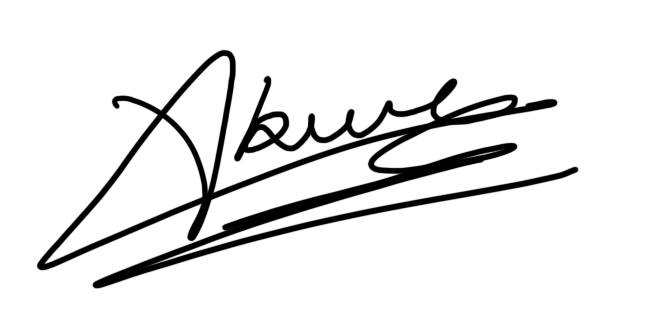
\includegraphics[width=0.2\textwidth]{images/Aditya_signature.png}
    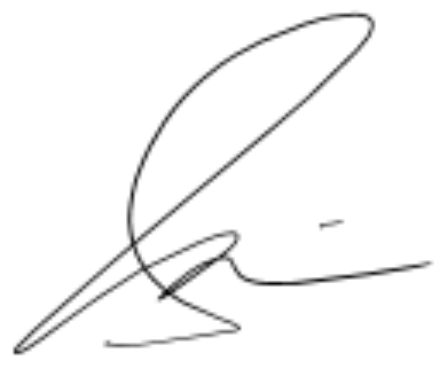
\includegraphics[width=0.1\textwidth]{images/sheikh_signature.png}
    
\includegraphics[width=0.1\textwidth]{images/Rizwan_sign.jpeg}
    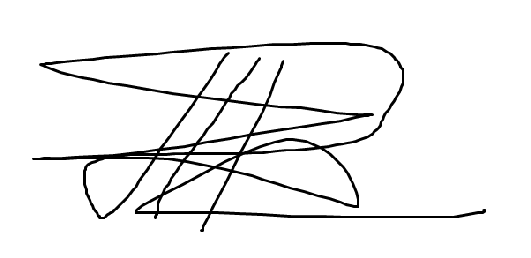
\includegraphics[width=0.2\textwidth]{images/mykyta_signature.png}
    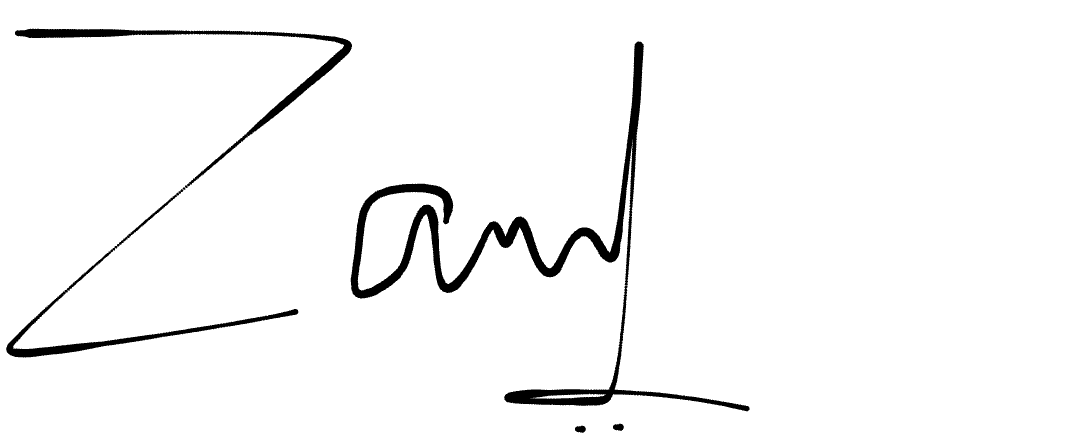
\includegraphics[width=0.2\textwidth]{images/Farhaad_signature.png}
\end{figure}

\end{document}